\input{../../Plantillas-Fomato/Tareas/tarea.tex}
\cabe{Geometría 3: Tarea 5}{Jhonny Lanzuisi, 1510759}
\pgfplotsset{compat=1.15}

\usepackage{mathrsfs}

\usetikzlibrary{arrows}
\begin{document}
		\tituloD{Geometría  3}{Sexta Tarea: Homotecias}
		\subsection*{Ejercicio 1}
		Sean $O$ un punto en el plano, $k$ una constante distinta de cero y $\ve v$
		un vector. La composición $T_{\ve v}\circ T_k$ de la homotecia con centro en $O$ y
		razón $k$ con la traslación determinada por el vector $\ve v$ es una homotecia.
		Determine su centro.
		\marginnote{
			\begin{minipage}{8cm}
				\begin{figure}[H]\hspace*{-2em}
					\begin{tikzpicture}[line cap=round,line join=round,>=triangle 45,x=1cm,y=1cm,scale=.55]
					\clip(-4.673940712150485,-3.901352956048242) rectangle (10.762249159621778,6.5012967401461275);
					\draw [->,line width=0.4pt] (1,1) -- (0,2);
					\draw [line width=0.4pt,domain=-4.673940712150485:10.762249159621778] plot(\x,{(--5-2*\x)/-0.5});
					\draw [line width=0.4pt,domain=-4.673940712150485:10.762249159621778] plot(\x,{(--8-2*\x)/-2});
					\begin{scriptsize}
					\draw [fill=black] (0,0) circle (1pt);
					\draw[color=black] (0.24774301508125135,0.19738690120806462) node {$O$};
					\draw[color=black] (0.775066271570366,1.5396642813621768) node {$\ve v$};
					\draw [fill=black] (3,2) circle (1pt);
					\draw[color=black] (3.2518876278071165,2.2427619566809978) node {$A$};
					\draw [fill=black] (4.5,3) circle (1pt);
					\draw[color=black] (4.817877904653578,3.2494699917965817) node {$A'$};
					\draw [fill=black] (3.5,4) circle (1pt);
					\draw[color=black] (3.923026317884171,4.096383100703343) node {$A''$};
					\draw [fill=black] (6,2) circle (1pt);
					\draw[color=black] (6.447786151983569,2.114926015713939) node {$B$};
					\draw [fill=black] (9,3) circle (1pt);
					\draw[color=black] (9.324094823742376,3.2494699917965817) node {$B'$};
					\draw [fill=black] (8,4) circle (1pt);
					\draw[color=black] (8.493161207456497,4.064424115461578) node {$B''$};
					\draw [fill=black] (2,-2) circle (1pt);
					\draw[color=black] (2.388995026279474,-1.9598446026110443) node {$O'$};
					\end{scriptsize}
					\end{tikzpicture}\caption{Determinación del centro de la homotecia $T$ con $k=3/2$.}
				\end{figure}
			\end{minipage}
		}[-7em]
		\begin{sol}
			Sean el punto $O$, el vector $\ve v$ y las transformaciones $T_{\ve v},T_k$ como en el enunciado. Para hallar el centro $O'$ de la homotecia $T = T_{\ve v}\circ T_k$ basta ver la intersección de dos rectas formadas por dos pares de puntos homólogos, es decir, si $A,B$ son dos puntos del plano (como se ve en la figura 1) y $A'',B''$ sus homólogos por $T$ entonces la intersección de las rectas $AA''$ y $BB''$ es $O'$, el centro de la homotecia $T$ buscado.
			
			Nótese que la construcción anterior puede fallar en dos casos, o $k=1$ o los puntos $A'',B''$ están sobre la recta $AB$. En el primer caso la homotecia $T_1$ es una traslación y no existe ningún punto invariante $O'$. En el segundo caso basta con tomar cualquier otro punto $C$ del plano exterior a la recta $AB$ y repetir la construcción anterior con $C$ en lugar de $B$.
		\end{sol}
	\subsection*{Ejercicio 2}
	Demostrar que el paralelogramo obtenido de unir los puntos medios de
	un cuadrilátero cualquiera es homotético a aquel que se obtiene de tra-
	zar por los extremos de las diagonales, paralelas a la otra. Determinar
	el centro de la homotecia.
	\marginnote{
		\begin{minipage}{8cm}
			\begin{figure}[H]\hspace*{-5em}
			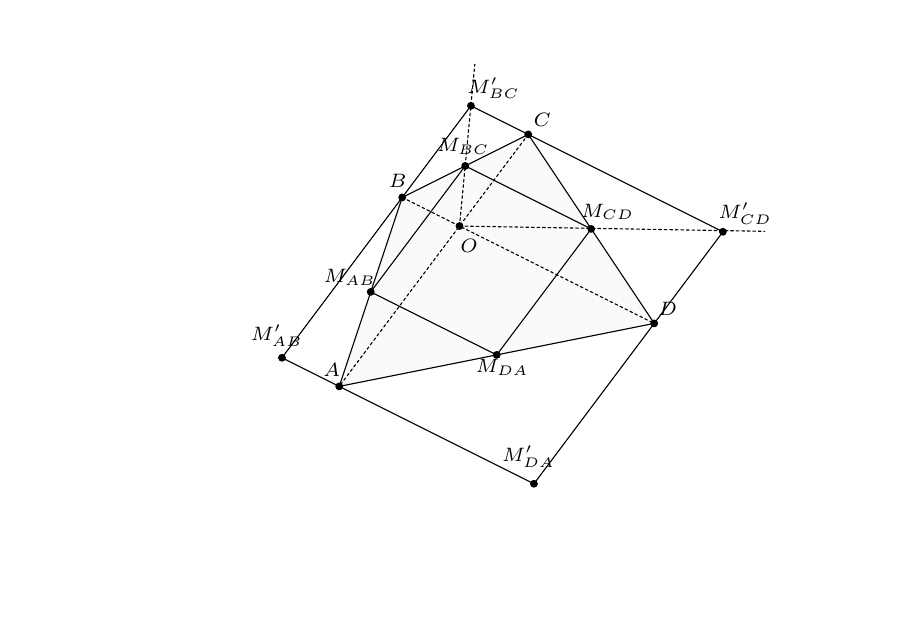
\begin{tikzpicture}[line cap=round,line join=round,>=triangle 45,x=1cm,y=1cm,scale=0.8]

			\clip(-4.946038597274534,-3.30523206234162) rectangle (8.408726701693757,5.694718465223968);

			\fill[line width=0.4pt,fill=black,fill opacity=0.02] (0,0) -- (1,3) -- (3,4) -- (5,1) -- cycle;

			\draw [line width=0.4pt] (0,0)-- (1,3);

			\draw [line width=0.4pt] (1,3)-- (3,4);

			\draw [line width=0.4pt] (3,4)-- (5,1);

			\draw [line width=0.4pt] (5,1)-- (0,0);

			\draw [line width=0.4pt] (2,3.5)-- (0.5,1.5);

			\draw [line width=0.4pt] (0.5,1.5)-- (2.5,0.5);

			\draw [line width=0.4pt] (2,3.5)-- (4,2.5);

			\draw [line width=0.4pt] (4,2.5)-- (2.5,0.5);

			\draw [line width=0.4pt,dash pattern=on 1pt off 1pt] (1,3)-- (5,1);

			\draw [line width=0.4pt,dash pattern=on 1pt off 1pt] (3,4)-- (0,0);

			\draw [line width=0.4pt] (2.090909090909091,4.454545454545454)-- (-0.9090909090909091,0.45454545454545453);

			\draw [line width=0.4pt] (-0.9090909090909091,0.45454545454545453)-- (3.090909090909091,-1.5454545454545454);

			\draw [line width=0.4pt] (3.090909090909091,-1.5454545454545454)-- (6.090909090909091,2.4545454545454546);

			\draw [line width=0.4pt] (6.090909090909091,2.4545454545454546)-- (2.090909090909091,4.454545454545454);

			\draw [line width=0.4pt,dash pattern=on 1pt off 1pt] (1.9090909090909092,2.5454545454545454)-- (2.152458744844366,5.114717621211607);

			\draw [line width=0.4pt,dash pattern=on 1pt off 1pt] (1.9090909090909092,2.5454545454545454)-- (6.754031016395965,2.4618538917049957);

			\begin{scriptsize}

			\draw [fill=black] (0,0) circle (1.5pt);

			\draw[color=black] (-0.12118032673630058,0.2546562031701139) node {$A$};

			\draw [fill=black] (1,3) circle (1.5pt);

			\draw[color=black] (0.9295051419195899,3.268464521156747) node {$B$};

			\draw [fill=black] (3,4) circle (1.5pt);

			\draw[color=black] (3.224423402404824,4.236201137024015) node {$C$};

			\draw [fill=black] (5,1) circle (1.5pt);

			\draw[color=black] (5.215195869331774,1.236217627835485) node {$D$};

			\draw [fill=black] (2,3.5) circle (1.5pt);

			\draw[color=black] (1.9663658017773764,3.807632064282796) node {$M_{BC}$};

			\draw [fill=black] (4,2.5) circle (1.5pt);

			\draw[color=black] (4.261284062262611,2.7707714044250094) node {$M_{CD}$};

			\draw [fill=black] (2.5,0.5) circle (1.5pt);

			\draw[color=black] (2.588482197692049,0.2961306295644254) node {$M_{DA}$};

			\draw [fill=black] (0.5,1.5) circle (1.5pt);

			\draw[color=black] (0.16914065802387968,1.7339107445672228) node {$M_{AB}$};

			\draw [fill=black] (2.090909090909091,4.454545454545454) circle (1.5pt);

			\draw[color=black] (2.45023410971101,4.733894253755753) node {$M'_{BC}$};

			\draw [fill=black] (6.090909090909091,2.4545454545454546) circle (1.5pt);

			\draw[color=black] (6.445603852363015,2.7431217868288016) node {$M'_{CD}$};

			\draw [fill=black] (1.9090909090909092,2.5454545454545454) circle (1.5pt);

			\draw[color=black] (2.063139463364103,2.2316038612989604) node {$O$};

			\draw [fill=black] (-0.9090909090909091,0.45454545454545453) circle (1.5pt);

			\draw[color=black] (-0.9921432810168413,0.8076485550942668) node {$M'_{AB}$};

			\draw [fill=black] (3.090909090909091,-1.5454545454545454) circle (1.5pt);

			\draw[color=black] (3.003226461635163,-1.1139998678421645) node {$M'_{DA}$};

			\end{scriptsize}

			\end{tikzpicture}
				\vspace{-5em}\caption{Dos paralelogramos homotéticos, con razón de la homotecia $k=2$.}
			\end{figure}
		\end{minipage}
	}
\begin{sol}
	Sean $ABCD$ un cuadrilátero y $M_{AB},M_{BC},M_{CD},M_{DA}$ los puntos medios de sus lados. Sean además $O$ la intersección de las diagonales del cuadrilátero $ABCD$ y $M'_{AB},M'_{BC},M'_{CD},M'_{DA}$ los vértices del paralelogramo formado al trazar por los extremos de las diagonales paralelas a la otra (como se ve en la figura 2).
	
	Queremos ver que los paralelogramos $M_{AB}M_{BC}M_{CD}M_{DA} $ y $M'_{AB}\linebreak M'_{BC}M'_{CD}M'_{DA}$  son hometéticos por la homotecia de centro en $O$.
	
	Como los segmentos $BO,M'_{BC}C$ y $OC,BM'_{BC}$ son pararelos por construcción, el cuadrilatero $BM'_{BC}CO$ es un paralelogramo. Las diagonales de este paralelogramo se intersectan en su punto medio, esto es, se intersectan en $M_{BC}$. De esto se sigue que los puntos $O,M_{BC},M'_{BC}$ son colineales y, además, 
	\[ \frac{OM'_{BC}}{OM_{BC}} = 2. \]
	
	Se obtiene un resultado similar al anterior sobre los tres puntos $O,M_{CD},M'_{CD}$ al considerar el paralelogramo $OCM'_{CD}D$. De esto se sigue que la imágen del segmento $M_{BC}M_{CD}$ por la homotecia de centro en $O$ y razón $k=2$ es el segmento $M'_{BC}M'_{CD}$.
	
	Una razonamiento análogo al anterior, considerando esta vez los paralelogramos $M'_{AB}BOA$ y $AODM'_{DA}$, se usa para demostrar que el segmento $M_{AB}M_{DA}$ es homotético al segmento $M'_{AB}M'_{DA}$.
	
	Entonces, por todo lo anterior, los paralelogramos $M_{AB}M_{BC}M_{CD}\linebreak M_{DA} $ y $M'_{AB}M'_{BC}M'_{CD}M'_{DA}$  son homotéticos por la homotecia de centro en $O$ y razón $k=2$.
\end{sol}
\subsection*{Ejercicio 3}
\marginnote{
	\begin{minipage}{8cm}
		\begin{figure}[H]\hspace*{-5em}
			\begin{tikzpicture}[line cap=round,line join=round,>=triangle 45,x=1cm,y=1cm,scale=.90]

			\clip(-3.9730625729394338,-6.1017229499964305) rectangle (14.689771532479112,6.270481736996938);

			\draw [line width=0.4pt] (0,0)-- (3,0);

			\draw [line width=0.4pt] (3,0)-- (4,0);

			\draw [line width=0.4pt] (4,0)-- (6,0);

			\begin{scriptsize}

			\draw [fill=black] (0,0) circle (1.5pt);

			\draw[color=black] (0.2080204242011774,0.29343354335728494) node {$A$};

			\draw [fill=black] (4,0) circle (1.5pt);

			\draw[color=black] (4.123034503341931,0.27442862064300944) node {$B$};

			\draw [fill=black] (3,0) circle (1.5pt);

			\draw[color=black] (3.210798213056707,0.31243846607156045) node {$C$};

			\draw [fill=black] (6,0) circle (1.5pt);

			\draw[color=black] (6.1755661564836855,0.31243846607156045) node {$D$};

			\draw[color=black] (1.6523945504861157,-0.352733828928083) node {$3u$};

			\draw[color=black] (3.6479114354850433,-0.352733828928083) node {$u$};

			\draw[color=black] (5.168305252627084,-0.3147239834995319) node {$2u$};

			\end{scriptsize}

			\end{tikzpicture}
			\vspace{-15em}\caption{Cuaterna armónica. Razones $r_a=2$,$r_b=1/2$. Longitud de segmentos en relación a la unidad de medida $u$.}
		\end{figure}
	\end{minipage}
}[-6em]
Sea $ABCD$ una cuaterna armónica. Sea $T_A$ la homotecia que transforma a $C$ en $D$ y $T_B$ la homotecia que transforma a $D$ en $C$. Muestre que $T=T_B\circ T_A$ es la simetría central con respecto a $C$.

\begin{sol}
	Sean $r_a$ la razón de $T_A$ y $r_b$ la razón de $T_B$.
	
	Por un lado, se sigue directamente de la definición de $T_A$ y $T_B$ que
	\[ T(C) = T_B(T_A(C)) = T_B(D) = C, \]
	y la homotecia $T$ deja invariante al punto $C$.
	
	Por otro lado, como $AB$ separa armónicamente a $CD$ (como en la figura 3) se cumple
	\[ \frac{AD}{AC} = -\frac{BD}{BC}, \]
	que implica,
	\[ \frac{BC}{BD}\frac{AD}{AC} = -1. \]
	
	Pero $BC/BD$ y $AD/AC$ son precisamente las razones $r_a$ y $r_b$. Luego el producto $r_ar_b = -1$ es la razón de $T$.
	
	Hemos descubierto entonces que $T$ es una homotecia de razón $-1$ y que deja invariante al punto $C$. Como todas las homotecias de razón $-1$ son simetrías centrales, se sigue que $T$ es la simetría central con respecto de $C$, como se buscaba.
\end{sol}
\marginnote{
	\begin{minipage}{8cm}
		\begin{figure}[H]\hspace*{-5em}
			\begin{tikzpicture}[line cap=round,line join=round,>=triangle 45,x=1cm,y=1cm,scale=.8,rotate=70]

			\clip(-3.2123530398700106,-2.4868352692957907) rectangle (8.886689462609366,5.666867286722839);

			\draw [line width=0.4pt] (0,0) circle (2cm);

			\draw [line width=0.4pt] (4,2) circle (1cm);

			\draw [line width=0.4pt] (1.898161100064201,2.5378855675644707) circle (1.170901217044908cm);

			\draw [line width=0.8pt,domain=-3.2123530398700106:8.886689462609366] plot(\x,{(--2.0125094597759463--0.6399414803471295*\x)/1.7849869648286933});

			\draw [line width=0.8pt,domain=-3.2123530398700106:8.886689462609366] plot(\x,{(-0--2*\x)/4});

			\draw [line width=0.4pt,domain=-3.2123530398700106:8.886689462609366] plot(\x,{(--8.76202167835014-2.78301967716079*\x)/-3.3669280842855667});

			\draw [line width=0.4pt,domain=-3.2123530398700106:8.886689462609366] plot(\x,{(-8.759754703311428-1.023342561666135*\x)/-4.245227423039342});

			\begin{scriptsize}

			\draw [fill=black] (0,0) circle (1pt);

			\draw[color=black] (0.24451624655266843,0.19975336091311335) node {$O'$};

			\draw[color=black] (-0.6948504073665378,1.4647671215242986) node {$c'$};

			\draw [fill=black] (4,2) circle (1pt);

			\draw[color=black] (4.202381081732257,2.191210667221811) node {$O$};

			\draw[color=black] (3.688860644256425,2.692206215978716) node {$c$};

			\draw [fill=black] (1.237544715437747,1.5711406930291463) circle (1pt);

			\draw[color=black] (1.3341815650989477,1.8029391169352096) node {$C_2$};

			\draw [fill=black] (3.0225316802664404,2.2110821733762758) circle (1pt);

			\draw[color=black] (2.887267766245369,2.4041337754434955) node {$C_1$};

			\draw[color=black] (1.6347788943530936,3.230776430892389) node {$s$};

			\draw [fill=black] (7.968693351479801,3.9843466757399004) circle (2pt);

			\draw[color=black] (7.9347979199712375,4.182667973530508) node {$H$};

			\end{scriptsize}

			\end{tikzpicture}
%			\vspace{-15em}\caption{Cuaterna armónica. Razones $r_a=2$,$r_b=1/2$. Longitud de segmentos en relación a la unidad de medida $u$.}
		\end{figure}
	\end{minipage}
}[-6em]
\end{document}